\documentclass{article}
\usepackage[utf8]{inputenc}
\usepackage{cite}
\usepackage[T1]{fontenc}
\usepackage{geometry}
\usepackage{amsmath}
\usepackage{amssymb}
\usepackage{comment}
\usepackage[round]{natbib}
\usepackage{graphicx}


%\geometry{
%    a4paper,
%    total={170mm, 257mm},
%    left=20mm,
%    top=10mm,
%}

\title{Master Thesis}
\author{Gaspard Ulysse Fragnière}
\date{August 2022}

\begin{document}

\maketitle

\section{State-of-the-art}

The problem of Acoustical Source Localization (ASL) is an important problem. It was many applications suach as smart assistant (e.g. Google Home, Alexa, ...), industrial applications, \textbf{TODO: add more?}. Traditionnaly this problem is tackled with methods based on the physics of sound propagation (e.g. TDoA, beamforming) or with statistcal inference (e.g.Sparse Bayesian Learning). 

The recent success of Deep Learning (DL) based method in other field of research (e.g. Computer Vision) led to believe that Deep Neural Networks (DNN) based approaches could provide state-of-the-art result in solving the ASL problem. \cite{castellini2021neural}, \cite{kujawski2019deep}, \cite{lee2021deep}, \cite{ma2019phased}, \cite{pinto2021deconvoluting} and \cite{xu2021deep} propose state-of-the-arts DL-based methods for Source Characterization. 


A common issue faced while implementing DL-based methods is that significant quantities of well structures data are required. In the litterature, the data has been obtained using the following approaches:

\begin{itemize}
    \item \textbf{Real Mesurement}: To create the different samples of such a dataset, sounds emitted with a loudspeaker or human voices are recorded in a real acoustic enviromnent. Eventhough such a method allows for the creation of perfectly realistic samples, it does not come without any issue. Indeed, it is very tedious and time consuming to record in different environment. Additionally, all the environment for measurement need to physically exists, which limits the quantity of possible samples. Moreover, to build a high quality data set, expensive equipment is required to have an accurate groundtruth (i.e. precisely identify the location of the sources). In the literature, \cite{he2018deep} and \cite{ferguson2018sound} have used such an approach.
    \item \textbf{Synthetic Data}: The sounds used are artificial (i.e. white noise, sine wave). The room acoustic is also simulated. Indeed the dry sound is convolved with a simulated Room Impulse Response (RIR) to mimic the effect of room acoustics (e.g. reverberation). Compared to real measurement, this approach allows sample in more diverse environment. Indeed RIR for rooms of arbitrary size, different source position as well as different dry signals can be used for the training. The issue with such a method is the important amount of time and storage required for the creation of the datasets. E.g. \cite{chakrabarty2017broadband}, \cite{perotin2018crnn} and \cite{adavanne2018direction} created their datasets in this way.
    \item \textbf{Semi-synthetic data}: The creation of such a dataset is similar the creation of synthetic dataset. The difference lies in the fact that the dry sound source used and the RIR are measured and not simulated. Then, the samples of such a dataset are generated by convolving dry sounds with RIR. This method is not the best suited, since it is very time-consuming to generate a data set with enough samples for training a DL-based algorithm. Indeed, measuring all the RIR lead to the issues faced with real measurement. \cite{takeda2016sound} use such an approach for to obtain their data.
\end{itemize}

Moreover it is to be noted that none of these methods are suitable for online data generation. Indeed, any of the above mentionned method do not allow for creating random sample while training DL-based algorithm. To use such datasets for training, they need to be fully created (and stored) before any training can occur. 

\subsection{DL-based data generation}

In the past years, DL-based approaches have shown to be able to learn and realistically reproduce very complicated data structures (e.g. generation of pictures of faces in the field of Computer Vision). Those breakthroughs lead to believe that similar data generation methods could be used to fix the above-mentionned issues (e.g. offline training, lack of variance in the different samples, ...).

Moreover, it is relevant to note that the data used for source characterization in \cite{castellini2021neural}, \cite{lee2021deep}, \cite{ma2019phased}, \cite{xu2021deep} is the Cross Power Spectra (CPS), i.e. a direct representation of the signals received in the array of microphone. Indeed those approaches do not use direct recording of microphone input but instead features extracted from the raw data. This is crucial because it means that recording, simulating or generating raw microphone data is no longer necessary, if features (e.g. CPS) could be generated directly. We therefore need to identify what acoustic quantities:
\begin{itemize}
    \item have already been generated using a DL approach
    \item are potential feature for a Source Characterization Algorithm.
\end{itemize}


\subsubsection{Generation of Signal}

\cite{neekhara2019expediting}, \cite{NEURIPS2019_6804c9bc}, \cite{engel2019gansynth} use Generative Adversial Network (GAN) to generate realistic audio waveform. \cite{neekhara2019expediting} and \cite{NEURIPS2019_6804c9bc} specifically focus on the generation of audio waveform conditioned on a spectogram (cGAN). On the other hand, \cite{engel2019gansynth} design a GAN to generate realistic audio waveform of single music notes played by an instrument. The data generated in those approaches is single-channel data, but maybe it could be extended to multi-channel to simulate the different signals recorded in an array of microphone. It is relevant to note that the GAN designed by \cite{neekhara2019expediting} is the one implemented in \cite{vargas2021improved} in order to compare the accuracy of a network for single source DoA estimation when trained with different sound classes.

\subsubsection{Generation of Impulse Response}

\cite{papayiannis2019data} introduce a GAN approach to generate artificial Acoustical Impulse Response (AIR) of different environment in order to generate data for a NN used for classification of acoustic environment.

\cite{ratnarajah2021fast} proposes a fast method (NN-based) for generating Room Impulse Response (RIR). The input paramaters of the networks used for creating the IR are the desired dimensions of the rectangular room, listener position, speaker position and reverberation time ($T_{60}$).

\textbf{TODO: is it worth mentionning both papers ?}

This is relevant for a problem at hand because if we are to be able to generate impulse responses with known source and listener position, we could simply convolve them with the dry source sounds. This way, we could generate raw microphone signal and use them to train a DL-based algorithm for source characterization.


\subsubsection{Generation of potential NN feature}

\cite{bianco2020semi} proposes an approach to generate another acoustic feature: the phase of the relative transfer function (RTF) between two microphones. In this paper a Variational Auto Encoder (VAE) is designed to simultaneously generate phases of RTF and classifying them by their Direction of Arrival (DoA).

\cite{gerstoft2020parametric} use a GAN to generate Sample Cross Spectra Matrices (CSM). for a given DoA. In their approach, the GAN is trained with data only coming from one DoA, making it unable to generate sample for different DoA. This approach could be extended by creating a conditional Generative Adversial Network (cGAN) taking as input the DoA. Such a GAN would receive a DoA as input and use it to produce a CSM corresponding to the received DoA.

\subsubsection{Other possible approaches to generate the data}

In \cite{hubner2021efficient} introduce a low complexity model-based method for generating samples of microphones phases. This method proposed is not based on DL. Indeed, it is based on a statistical noise model, a deterministic direct-path model for the point source, and a statistical model. The claim of this paper is that the low complexity of the proposed  model makes it suited for online training data generation. 

\cite{vera2021acoustic} introduce a CNN for denoising (i.e. removing the effects of reverberation and multipath effects) on the Generalization Cross Correlation (GCC) matrix of an array of microphone. More specifically than a CNN, the network used has a encoder-decoder structure. This means that a possible approach to create the data we want, would be to attempt to invert network proposed. With this we could realistically add noise to GCC matrices and hence making it suitable for training.

\section{Our approach}

We decided that it made sense to try to generate the Cross Spectral Matrix (CSM), as done in \cite{gerstoft2020parametric} and extend his work to create a network to generate CSM, conditionally on Direction of Arrival (DoA). Indeed, such a network would allow us to have the online generation of labeled data required to train the network \textbf{TODO: find name of network for Source Characterization}. By providing a DoA (i.e. a label) to the network, we would generate the corresponding CSM data.

More specifically than the CSM, we thought it would make more sense to generate separately the eigenvalues and eigenvectors its eigendecomposition. A CSM $\mathbf{\hat{C}}$ can be decomposed as :

\begin{equation}
    \mathbf{\hat{C}} = \mathbf{V} \mathbf{\Lambda} \mathbf{V}^H
\end{equation}

where $\mathbf{V} = [\mathbf{v}_1^T, \dots, \mathbf{v}_M^T] \in \mathbb{C}^{M \times M}$, $\mathbf{v}_i$ being the $i$th eigenvector and where $\mathbf{\Lambda} \in \mathbb{R}^{M \times M}$ is a diagonal matrix, where $\lambda_{ii}$ is the $i$th eigenvalue, corresponding to the $i$th eigenvector.

Indeed, since we choose a Generative Adversial Approach, the data will be generated using two networks: a generator and a discriminator/critic. Those two network are competing against each other: the goal of the generator is to produce data realistic enough so that discriminator can not tell it is fake. The goal of the discriminator is to tell whether a given input is real or has been generated. Both the generator and the discriminator have to be trained simultaneously until convergence. A typical issue occuring during the training, is that the discriminator becomes too good at discerning real from fake sample and hence the generator does not improve anymore.

Generating the eigenvalues and eigenvectors instead of the CSM is done in order to help the generator. This allow to normalize all the eigenvectors before feeding them to the discriminator, whether they are real or generated. The eigenvalues can also be scaled the biggest of them is equal to one. \textbf{TODO: develop on that} 

\section{Data generation}

\textbf{TODO: fill this section if necessary} 

\section{Generation of Eigenvalues}



\subsection{GAN approach}

As an attempt to generate the data, the first approach was to build a GAN network. The architecture used was taken from \cite{eriklindernoren}. The architecture of the generator here were regular perceptron and activation function. \textbf{TODO: Are more details about the architecture required?}. We show in Fig.\ref{fig:GAN_evals_loss_acc} the losses and accuracies of the generator and discriminator plotted as function of the trainings epochs. It can be easily observed that the typical non-convergence scenario is happening. Indeed the loss of the discriminator quickly decreases to zero, while its accuracy reaches one. On the other hand, the loss of the generator increases steadily while its accuracy remains at zero.

\begin{figure}
    \centering
    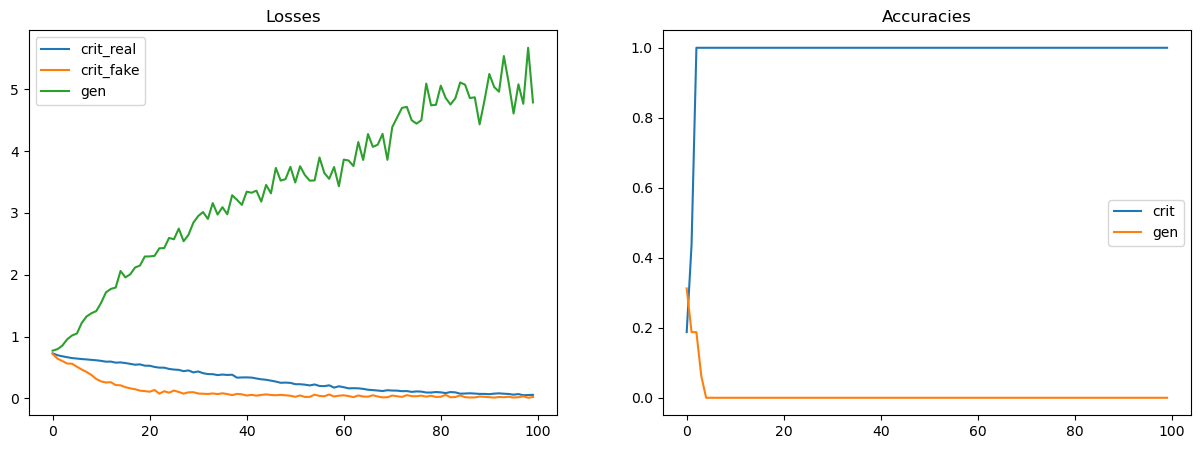
\includegraphics[width=\textwidth]{../figs/GAN_evals_loss_acc.png}
    \caption{GAN: Loss and Accuracy of the generator and dsicriminator plotted as a function of the training epochs}
    \label{fig:GAN_evals_loss_acc}
\end{figure}

For a reference, in a convergening GAN, the following behaviour is expected to be observed:

\begin{itemize}
    \item Discriminator loss on real and fake samples is expected to sit around 0.5.
    \item Generator loss on fake samples is expected to sit between 0.5 and perhaps 2.0.
    \item Discriminator accuracy on real and fake samples is expected to sit around 80 percent.
    \item Variance of generator and discriminator loss is expected to remain modest.
    \item The generator is expected to produce its highest quality samples during a period of stability.
    \item Training stability may degenerate into periods of high-variance loss and corresponding lower quality generated samples.
\end{itemize}

\subsection{DCGAN approach}

As an attempt to improve the above-mentionned performances, the perceptron layers of the generator and discriminatort were replaced by convolutional layert and both networks were deepened. The implementation was the one used in the DCGAN in \cite{eriklindernoren}. The observed performance are then the ones of Fig.\ref{fig:DCGAN_evals_loss_acc}. As for the GAN, the same non-convergence pattern can be observed.

\begin{figure}
    \centering
    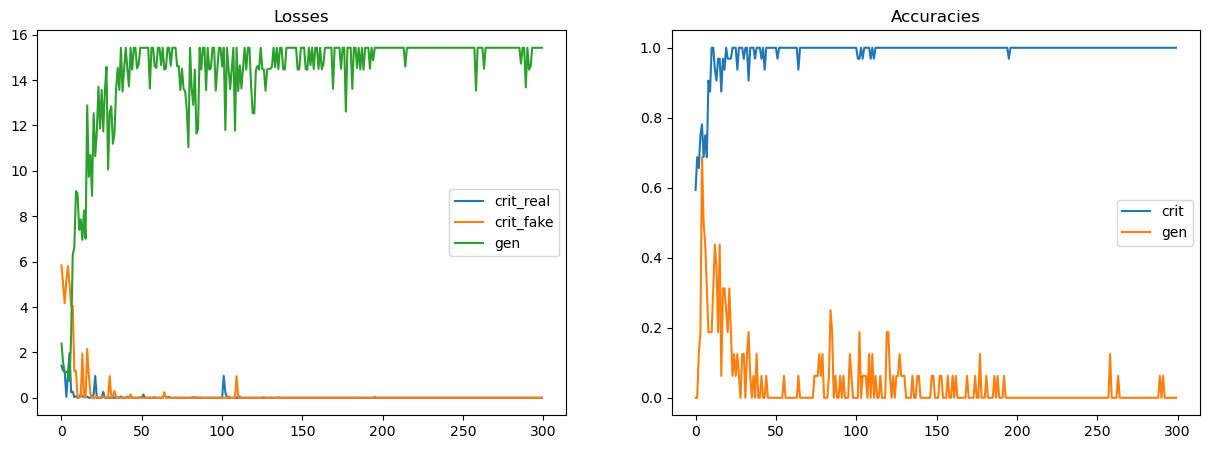
\includegraphics[width=\textwidth]{../figs/DCGAN_evals_loss_acc.png}
    \caption{DCGAN: Loss and Accuracy of the generator and dsicriminator plotted as a function of the training epochs}
    \label{fig:DCGAN_evals_loss_acc}
\end{figure}

\subsection{WGAN-GP approach}

In order to fix the convergence issue experienced by teh models above, we implement the Wasserstein GAN (WGAN). More specifixcally we implement its imporved version, Wasserstein GAN with Gradient Penalty (WGAN-GP). \textbf{TODO: finish writing this section once the WGAN-GP has been successfully implemented}

\section{Generation of Eigenvectors}

\textbf{TODO: write this section}


\section{Networks explained}

\subsection{GAN}

\textbf{TODO: include explanation about GAN basic principle}

\subsection{DCGAN}

\textbf{TODO: include explanation about DCGAN basic principle}

\subsection{WGAN}

\cite{arjovsky2017wasserstein} introduce a new type of Generative Adversial Network, namely the Wasserstein GAN (WGAN). The claim is that WGAN improves the stability in learning and get rid of typical problem of the traditional GAN approach such as Mode Collapse or Convergence failure. \textbf{TODO: here need to explain mode collapse ?}. 

\begin{comment}
More specifically, \cite{arjovsky2017wasserstein} provides the following insights:

\textbf{TODO}: Here needs to state the problem that the Earth Mover distance (distance between probability) try to solve.

\begin{itemize}
    \item Analyses how the Earth-Mover (EM) distance, also known as Wasserstein distance behaves compared to other distance between probability distribution (e.g. Kullback-Leibler distance)
    \item Define a GAN that minimizes the an approximation of the EM distance, namely the WGAN.
    \item Show that unlike traditional GANs, WGANs do not need to maintain a balance when training the discriminator and generator. Indeed in regular GAN approach, it was crucial to avoid the discriminator to become too good before the generator, since this would prevent the generator to learn any distribution. 
\end{itemize}
\end{comment}

\subsubsection{The Earth-Mover or Wasserstein distance}

%\textbf{TODO}: Understand and explain loss function structure + Check if the loss function used is the same as the one used in the original Wasserstein paper.

The goal of WGAN, remains the same as GAN, namely approximation of of the probability distribution $P_r$ of some data by distribution $P_{\theta}$. For this reason, it is necessary to have metrics to quantify distance between probability distributions $P_r$ and $P_m$ (e.g. Kullback-Leibler divergence, Jensen-Shannon divergence, ...). In WGAN, the distance used is the Earth-Mover (EM) distance or Wasserstein-1, defined as 

\begin{equation}
    W(\mathbb{P}_r, \mathbb{P}_m) = \inf_{\gamma \in \Pi(\mathbb{P}_r, \mathbb{P}_m)} \mathbb{E}_{(x,y) \sim \gamma} [||x-y||]
\end{equation}

Where $\Pi(\mathbb{P}_r, \mathbb{P}_m)$ is the set of all joint distribution $\gamma(x,y)$ whose marginals are respectively $\mathbb{P}_r$ and $\mathbb{P}_m$. Informally, $\gamma(x,y)$ shows how much "mass" must be carried to trasnform $\mathbb{P}_r$ into $\mathbb{P}_m$. The EM distance is then "the cost" of the optimal "transport". Unfortunately the EM distance is intractable, due to the infinum part in its equation, but the Kantorovich-Rubinstein duality tells us that

\begin{equation}
    W(\mathbb{P}_r, \mathbb{P}_{\theta}) = \sup_{||f||_L \leq 1} \mathbb{E}_{x \sim \mathbb{P}_r} [f(x)] - \mathbb{E}_{x \sim \mathbb{P}_{\theta}} [f(x)] 
\end{equation}

Where the supremum is over 1-Lipschitz function. It is important to note that if we replace $||f||_L \leq 1$ by $||f||_L \leq K$, i.e. consider also the K-Lipschitz function, then we obtain $K \cdot W(\mathbb{P}_r, \mathbb{P}_{\theta})$. Hence, for a family of functions $\{f_w\}_{w \in \mathcal{W}}$ (all functions being K-Lipschitz), we can consider solving the optimization problem:

\begin{equation}
    \max_{w \in \mathcal(W)}  \mathbb{E}_{x \sim \mathbb{P}_r}[f_w(x)] - \mathbb{E}_{z \sim p(z)}[f_w(g_{\theta}(z))]
\end{equation}

Note: we can approximate the solution of the above mentionned problem with a Neural Network with weights $\mathcal{W}$. $\mathcal{W}$ need to be compact to assure that the function $f_w$ are K-lpischitz. Therefore in order to have $\mathcal{W}$ being compact, \cite{arjovsky2017wasserstein} proposes to simply clip the weights, such that they lay in a small box (e.g. $[-0.01, 0.01]^l$)


\subsubsection{Necessary changes to turn a GAN into a WGAN}

Implementation of a WGAN requires a few changes from implementation of a regular GAN, i.e. 

\begin{itemize}
    \item Use a linear activation function in the output layer of the "discriminator" model (instead of sigmoid). The "discriminator" then becomes a critic that quantify the realness of a sample, instead of discriminating between real or fake.
    \item Use Wasserstein loss to train the critic and generator models that promote larger difference between scores for real and generated images. 
    \item Constrain critic model weights to a limited range after each mini batch update (e.g. [-0.01,0.01]). As seen above, this is to ensure, that the function estimated in the for approximting the Wasserstein distance are K-lipschitz, a necessary condition.
    \item Update the critic model more times than the generator each iteration (e.g. 5). Contrary as in a GAN, this is not a issue. Indeed, switching to the EM distance, allow for more stability when training the two networks in the WGAN. Moreover, the fact that the EM distance is continuous and differentiable means that we should train the critic until optimality.
    \item Use the RMSProp version of gradient descent with small learning rate and no momentum (e.g. 0.00005).
    
\end{itemize}



\subsection{WGAN-GP}

As we have seen above, WGAN improve the stability in training the critic ($\approx$ discriminator). But sometimes, they only generate poor sample or fail to converge. This is due to the weight clipping happening while training the critic. In order to remedy to this, \cite{DBLP:journals/corr/GulrajaniAADC17} propose to replace weight clipping by the introduction of a penalization of the norm of gradient of the critic with respect to its input. The issue is that trying to orient the critic to 1-Lipschitz function by weight clipping, biases the critic for too simple function.

\textbf{TODO: Explain more formally the Gradient Penalty}


% ========================================================================

% Bibliography
%\addbibresource{mybib.bib}
\bibliography{../mybib}
\bibliographystyle{plainnat} 


\end{document}